\section{Understanding line up automation} \label{sec:understanding_automated_line_up}
This section describes basic concepts of the line up automation (LUA) system. The automated line-up system is a system that aligns two pipes together. The system consists of a U-Frame, laser line scanners, Line up Car Assemblies (LCAs) and a sub-frame. The U-Frame houses the laser line scanners and is mounted on the sub-frame. The sub-frame is responsible for the U-Frame's movements. The LCAs are devices that control the new joint's position and orientation. The laser line scanners are sensors that detect the new joint's position.

\subsection{The U-frame} \label{ssec:U-frame}
Figure \ref{fig:U-frame} shows the U-Frame. The U-frame is a part of the automated line-up system. It is precisely machined to ensure that the positions of the laser line scanners are known as accurately as possible.
\begin{figure}[H]
    \centering
    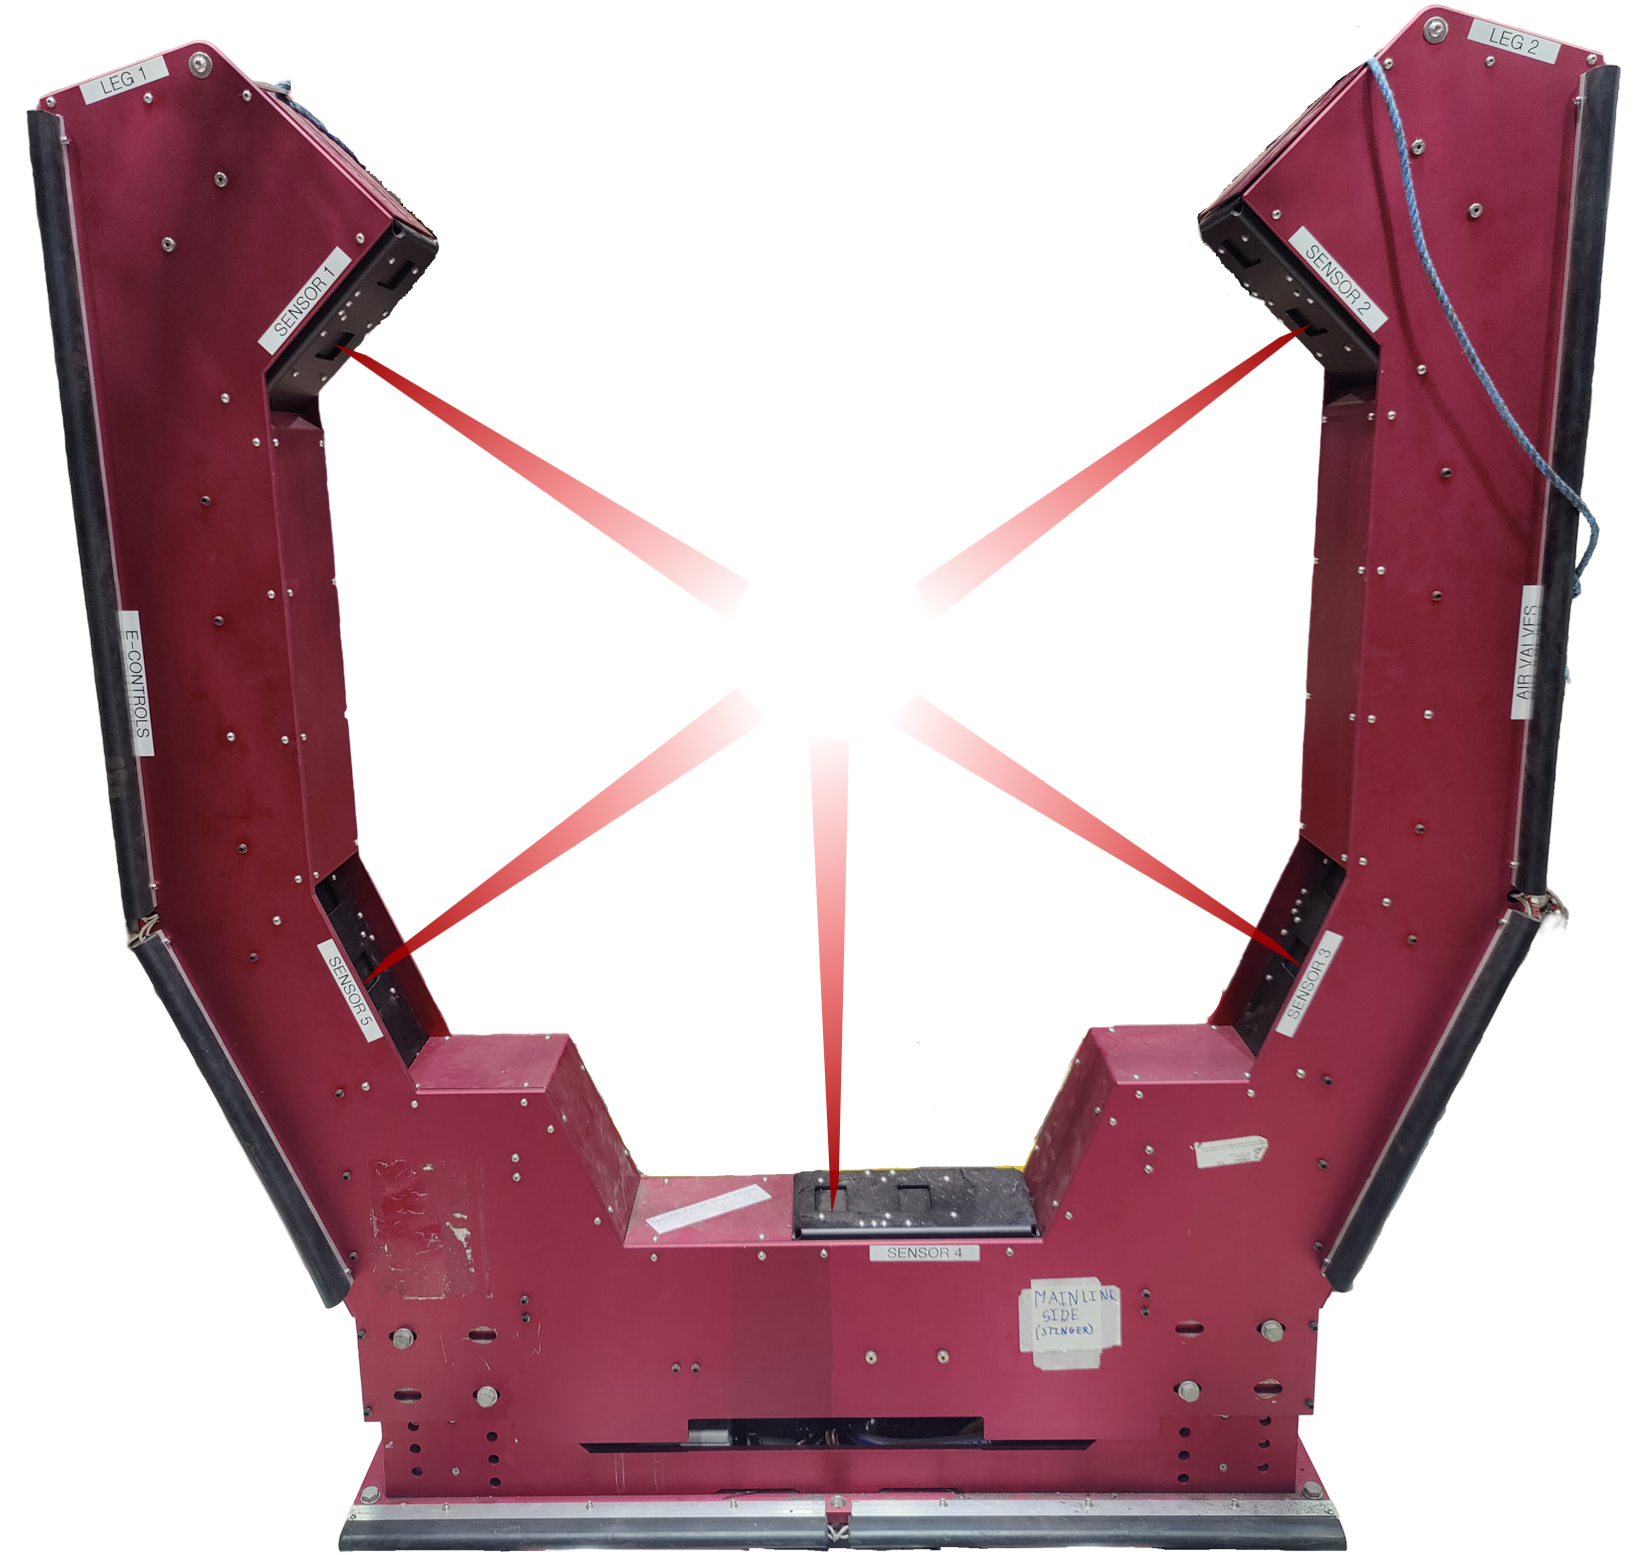
\includegraphics[width=0.7\textwidth]{images/u_frame_lasers.png}
    \caption{The U-Frame. Most importantly, the U-frame houses five laser line scanners that are used to detect pipes and other objects like the ILUC. The U-Frame is mounted on an interface frame, which in turn is mounted on the sub-frame (not visibile here). The sub-frame is responsible for the U-Frame's movements.}
    \label{fig:U-frame}
\end{figure}

The U-Frame is given a right-handed cartesian coordinate system. The origin of the coordinate system is at the center of the U-Frame. The $x$-axis points towards the new joint, the $y$-axis points left (seen from the main line) and the $z$-axis points upwards. 

\subsection{Laser line scanners} \label{ssec:laser_line_scanners}
The laserline scanners measure in 2 dimensions, width ($x$-direction) and depth ($z$-direction). The scanners each generate 4192 data points in any one measurement. The frequency of the measurements in only limited by how fast the laser line scanner runs (see section \ref{ssec:code_flow}). The maximum scanning frequency of the lasers lies anywhere between 600 and 9000 Hz \cite{gocator2650datasheet}.

The lasers measure in their respective coordinate systems. These measurements are then transformed to the U-Frame's coordinate system. To perfrom this transformation, the laser line scanners angles with respect to the U-Frame's coordinate system are needed. These angles are 
\begin{align}
    \phi_1    & = \frac{\pi}{4},                              \\
    \phi_2    & = \frac{3\pi}{4},                             \\
    \phi_3    & = \frac{9\pi}{8},                             \\
    \phi_4    & = \frac{15\pi}{8},                            \\
    \phi_5    & = \pi,
    \label{eq:laser_angles}
\end{align}
where the angles are measured from the $z$-axis in the $y$-$z$ plane with positive rotation defined by the right hand rule applied to the $x$-axis. In this simple case the angles are the same as the angles of the laser line scanners in the U-frame.

An important aspect of the laser line scanners is their Field of View (FOV).
The FOV is the area in which the laser line scanners can detect objects. Figure \ref{fig:lls_fov} gives the FOV of the laser line scanners.
\begin{figure}[H]
    \centering
    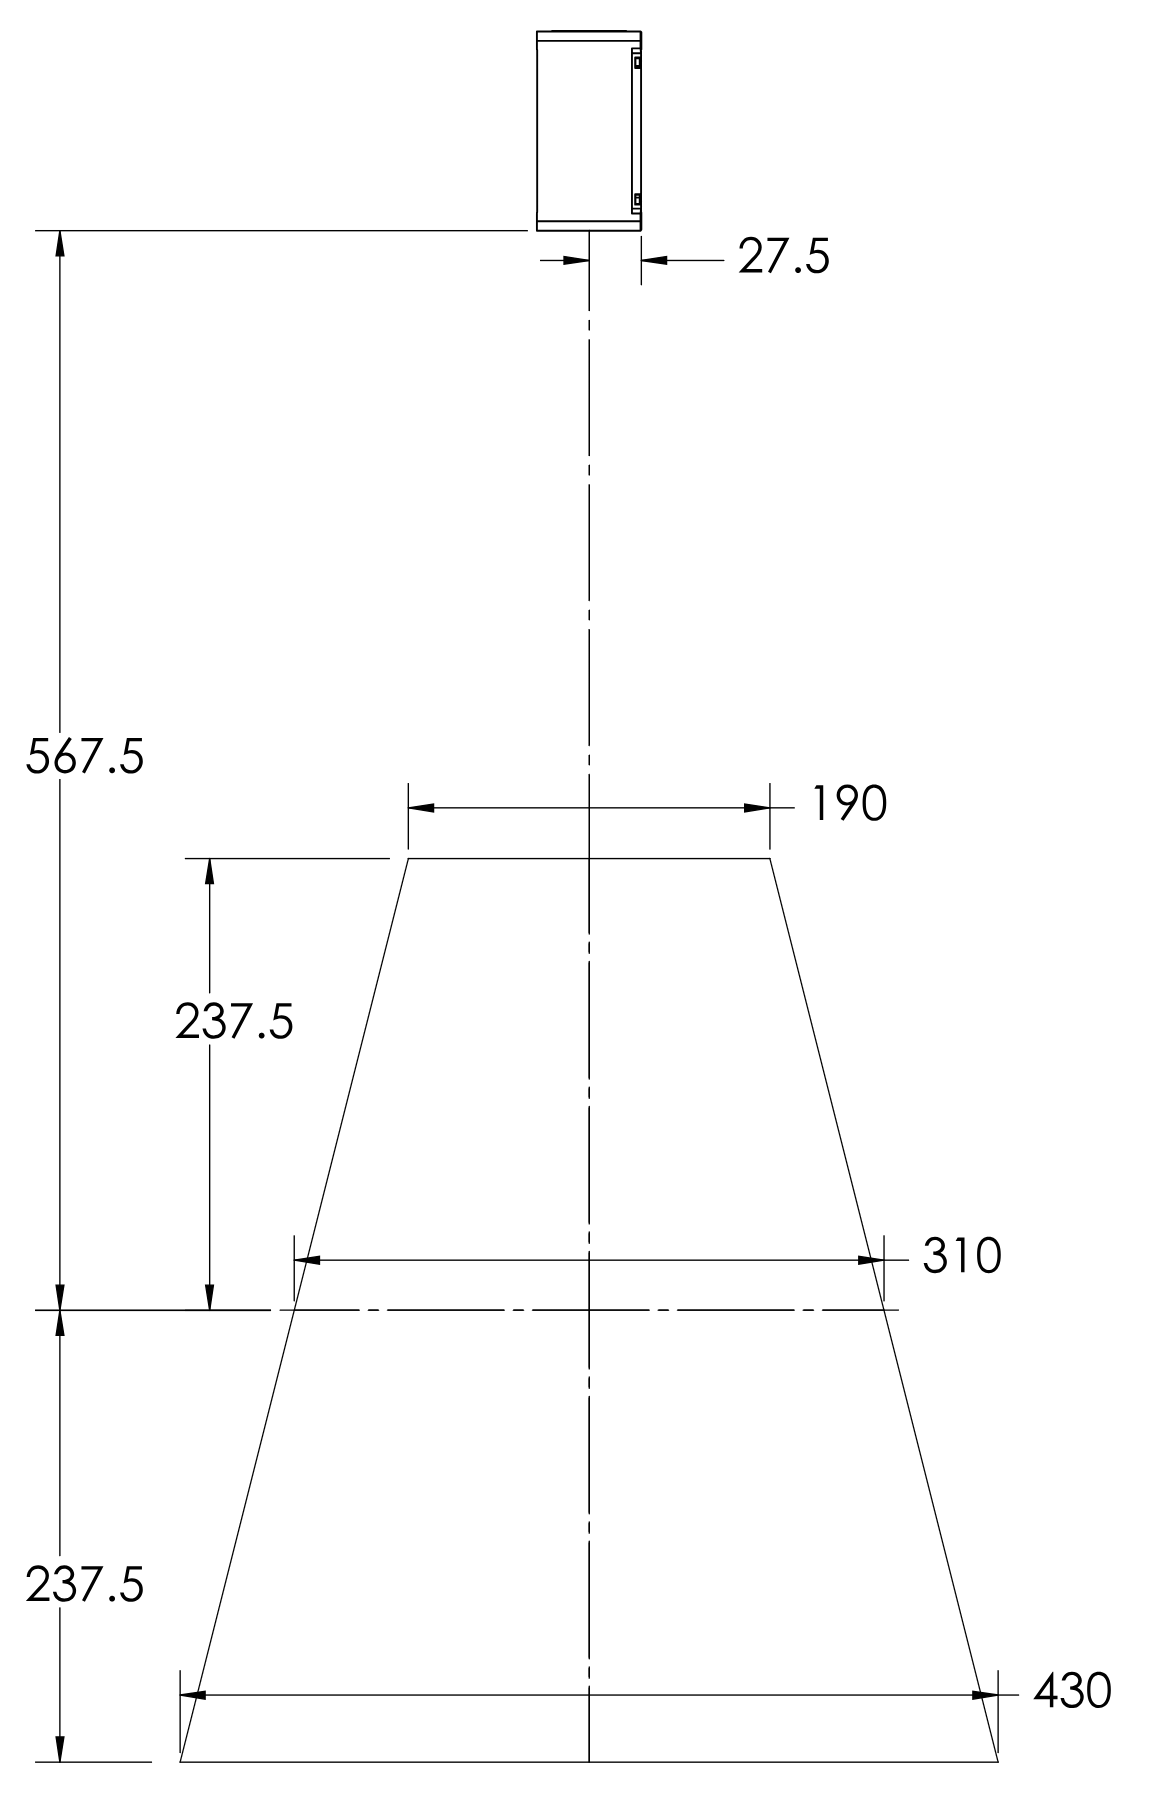
\includegraphics[width=0.5\textwidth]{images/laser_line_scanner_fov.png}
    \caption{Field of View (FOV) of the laser line scanners. Measurements are in millimeters \cite{gocator2650FOV}.}
    \label{fig:lls_fov}
\end{figure}
From figure \ref{fig:lls_fov} it can be seen that the FOV of the laser line scanners is limited. In particular, the width of the frame itself is $\sim 20$ cm, which means the laser line scanners can see $\sim 10$ cm beyond either side of the frame. This is why it is necessary for the U-Frame to move.

Depending on the distance of an object to a laser line scanner, the accuracy its measurement can vary. For an object close to the laser line scanners the resolution is $47 \mu m$ in the $x$-direction. For an object further away from the laser line scanners the resolution is $104 \mu m$ in the $x$-direction \cite{gocator2650datasheet}.

In terms of the $z$-direction, an indication of accuracy is given by the repeatability. This value is determined by using a flat target and calculating the 95\% confidence variation of the average height over 4096 measurement frames. $z$ values are averaged over the full FOV. The repeatability comes out to be $2 \mu m$ \cite{gocator2650datasheet}.

\newpage
\subsection{Order of operations automated line-up} \label{ssec:oop_lua}
Figure \ref{fig:oop_lua} shows the order of operations during automated line-up.
\begin{figure}[H]
    \centering
    \begin{subfigure}{0.7\textwidth}
        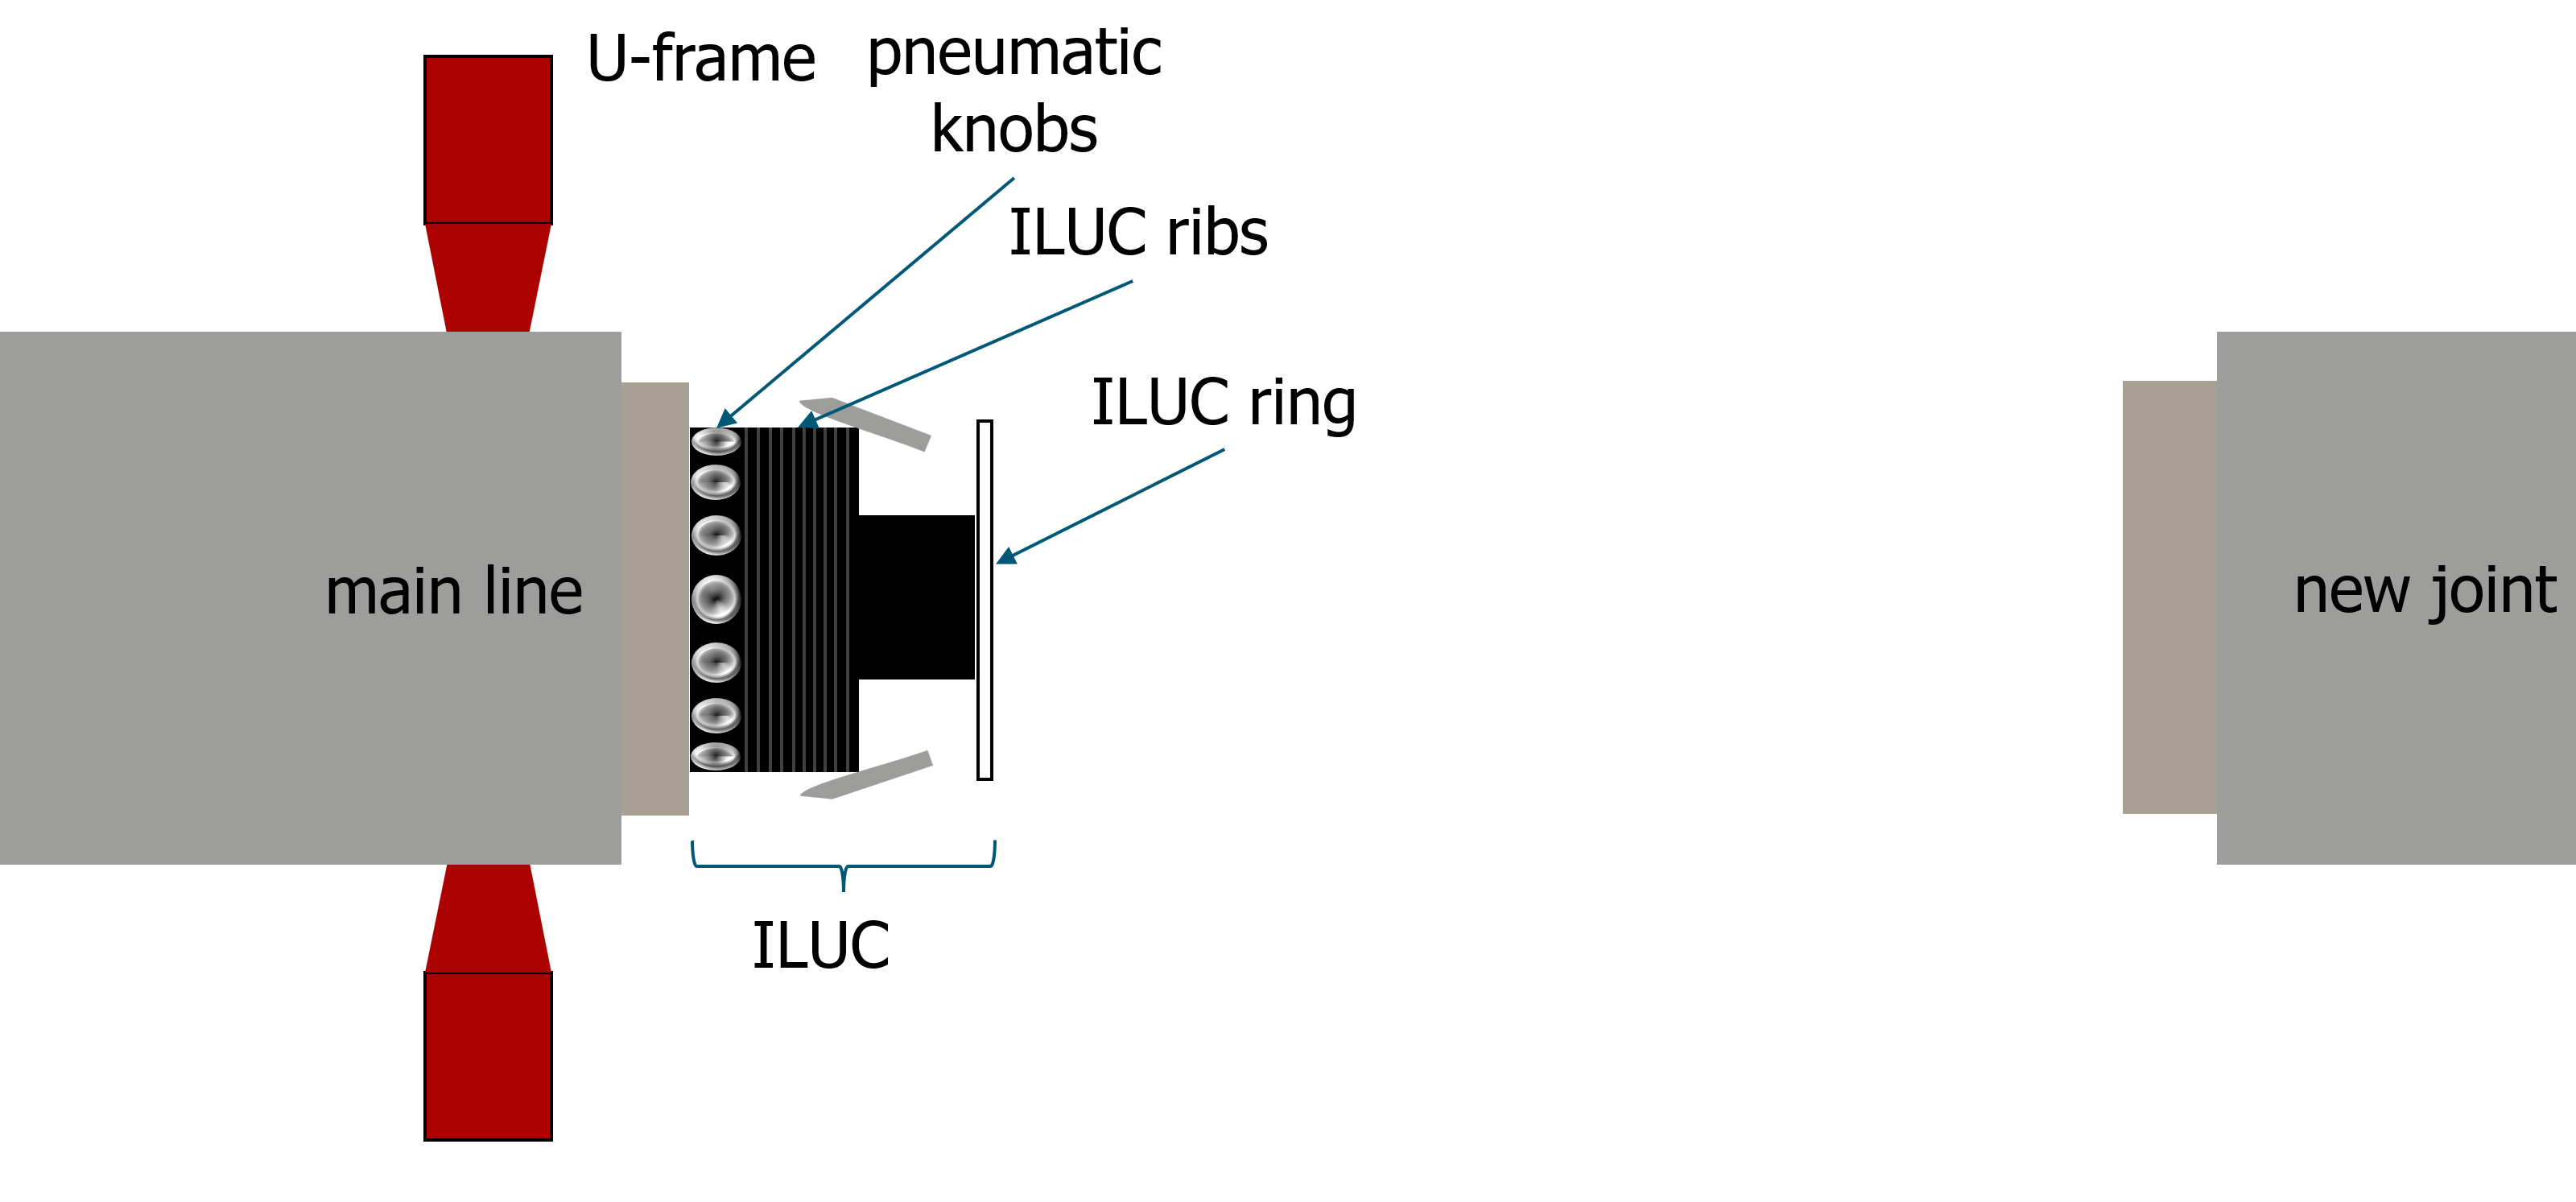
\includegraphics[width=\textwidth ]{images/lua_oop_intro.png}
        \caption{Initial state of automated line up. The main line is depicted on the left,
            while the new joint is depicted on the right. The U-Frame is in its starting position. The ILUC
            sits in the main line. Visible parts of the ILUC are its pneumatic knobs, black ribbed cylinder (ILUC ribs)
            and white ring (ILUC ring).}
        \label{fig:oop_intro}
    \end{subfigure}
    \begin{subfigure}{0.7\textwidth}
        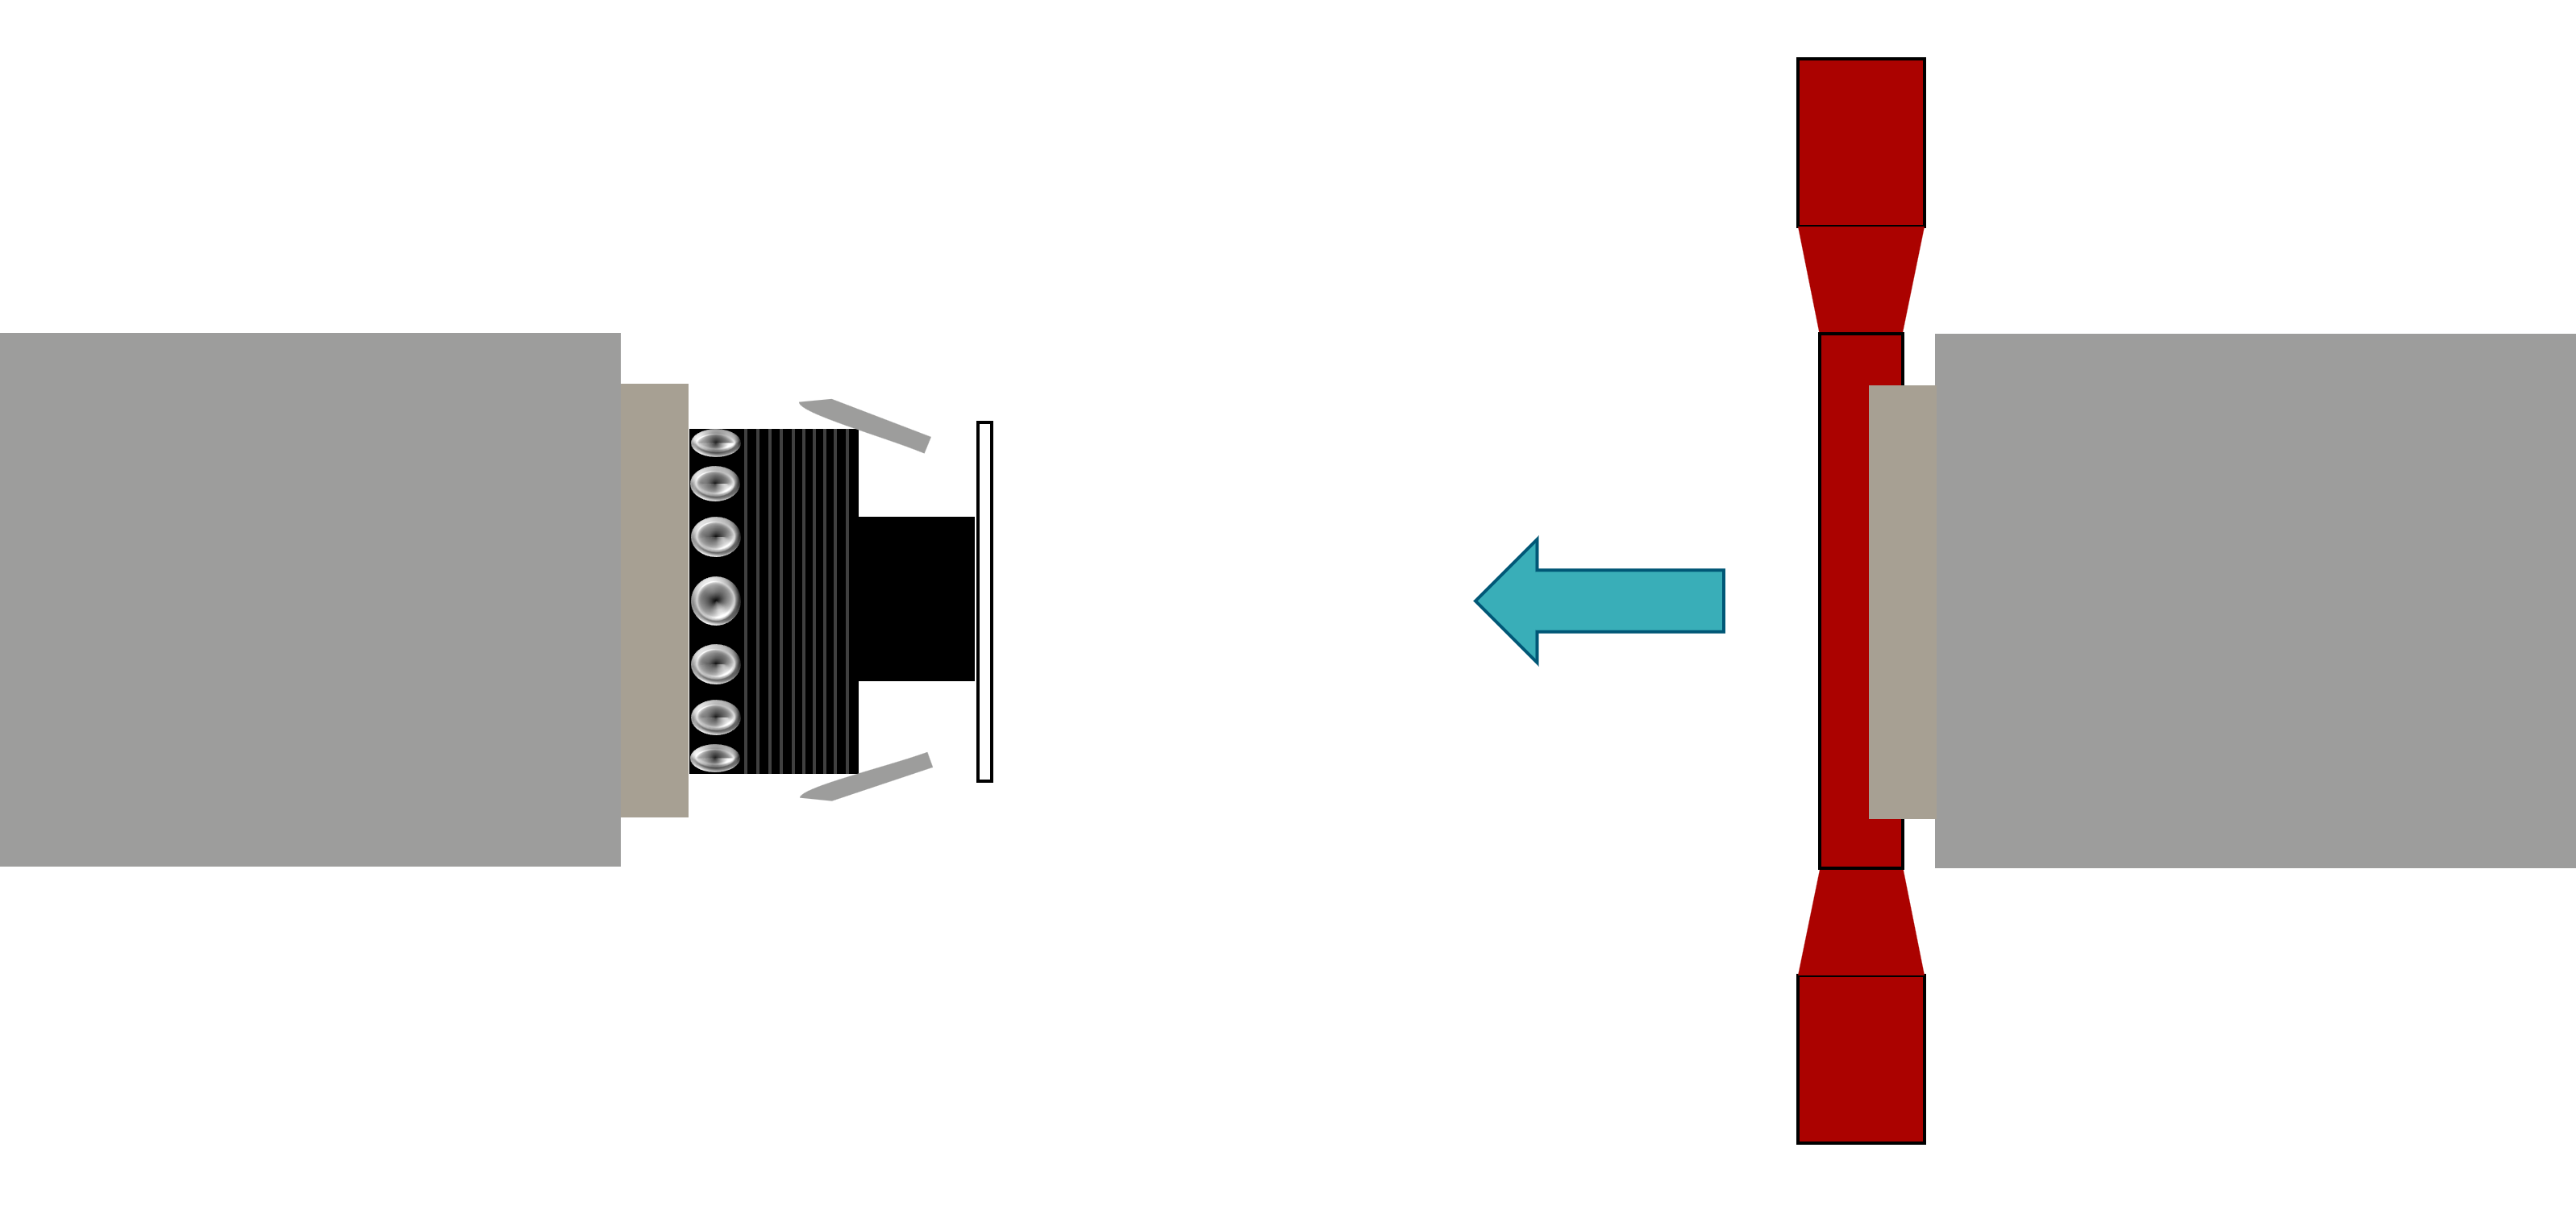
\includegraphics[width=\textwidth ]{images/lua_oop_track_new_joint.png}
        \caption{The U-Frame moves to the right until it encounters the new joint, which is moved towards the main line.
            The U-Frame reverses direction and tracks the new joint upon its recognition by the laser line scanners.}
        \label{fig:oop_track}
    \end{subfigure}
    \begin{subfigure}{0.7\textwidth}
        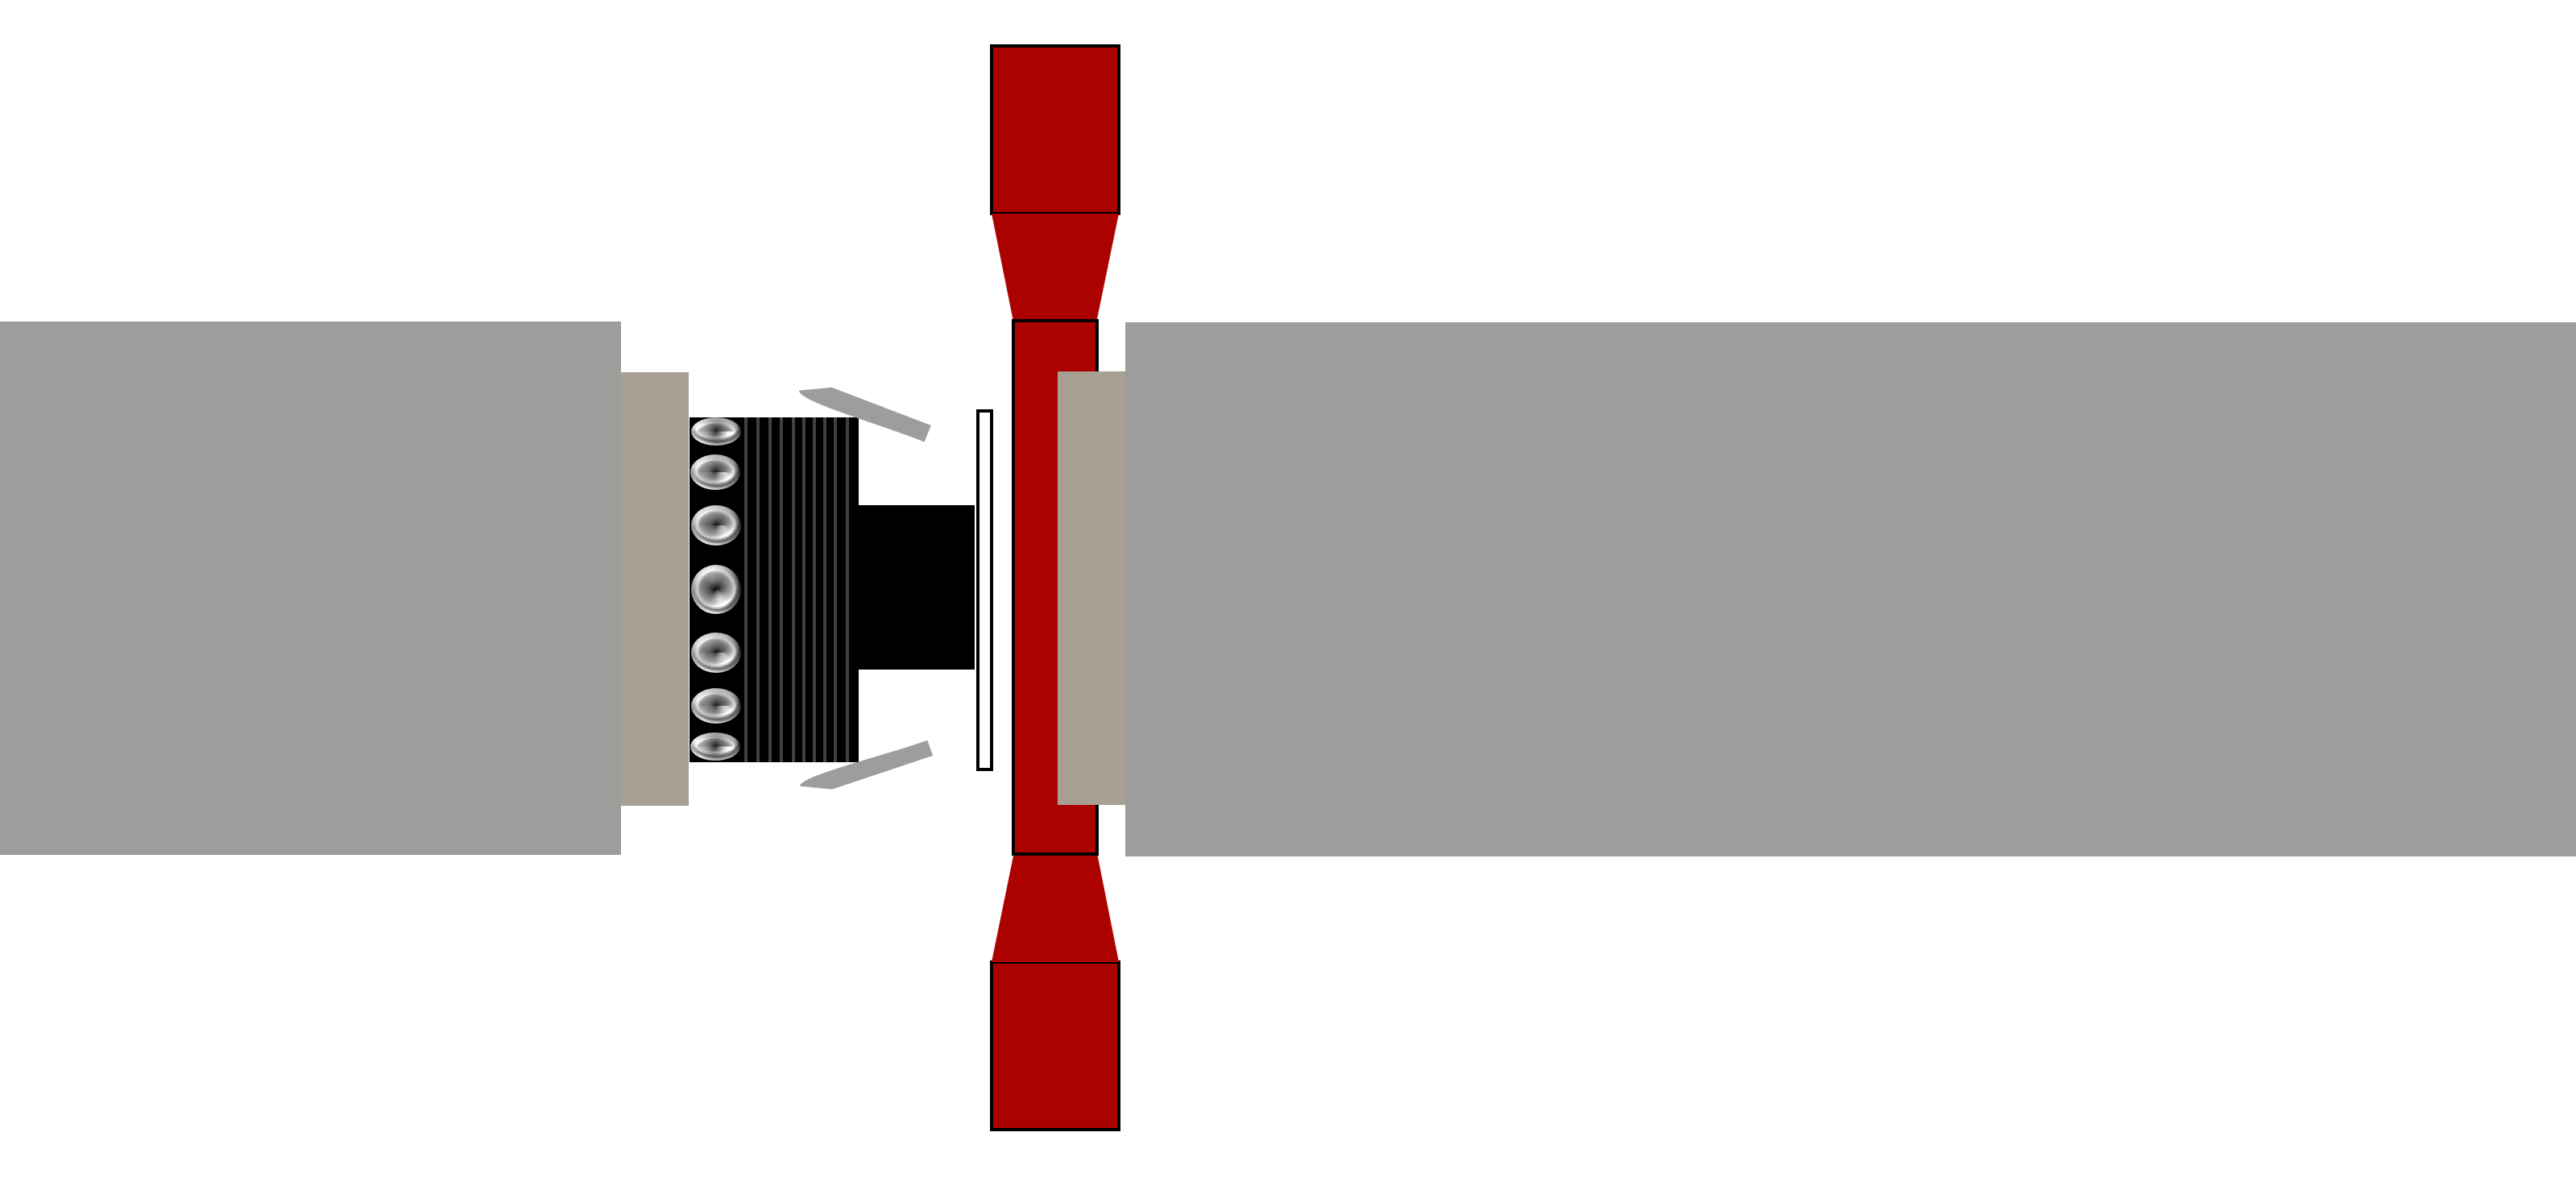
\includegraphics[width=\textwidth ]{images/lua_oop_ILUC_ring.png}
        \caption{The laser line scanners detect the ILUC ring. The first adjustments are made to the new joint's position.
            This is done to ensure that the new joint is shifted over the ILUC ring and other parts of the ILUC.}
        \label{fig:oop_ILUC_ring}
    \end{subfigure}
\end{figure}
\begin{figure}[H]
    \ContinuedFloat\centering
    \begin{subfigure}{0.7\textwidth}
        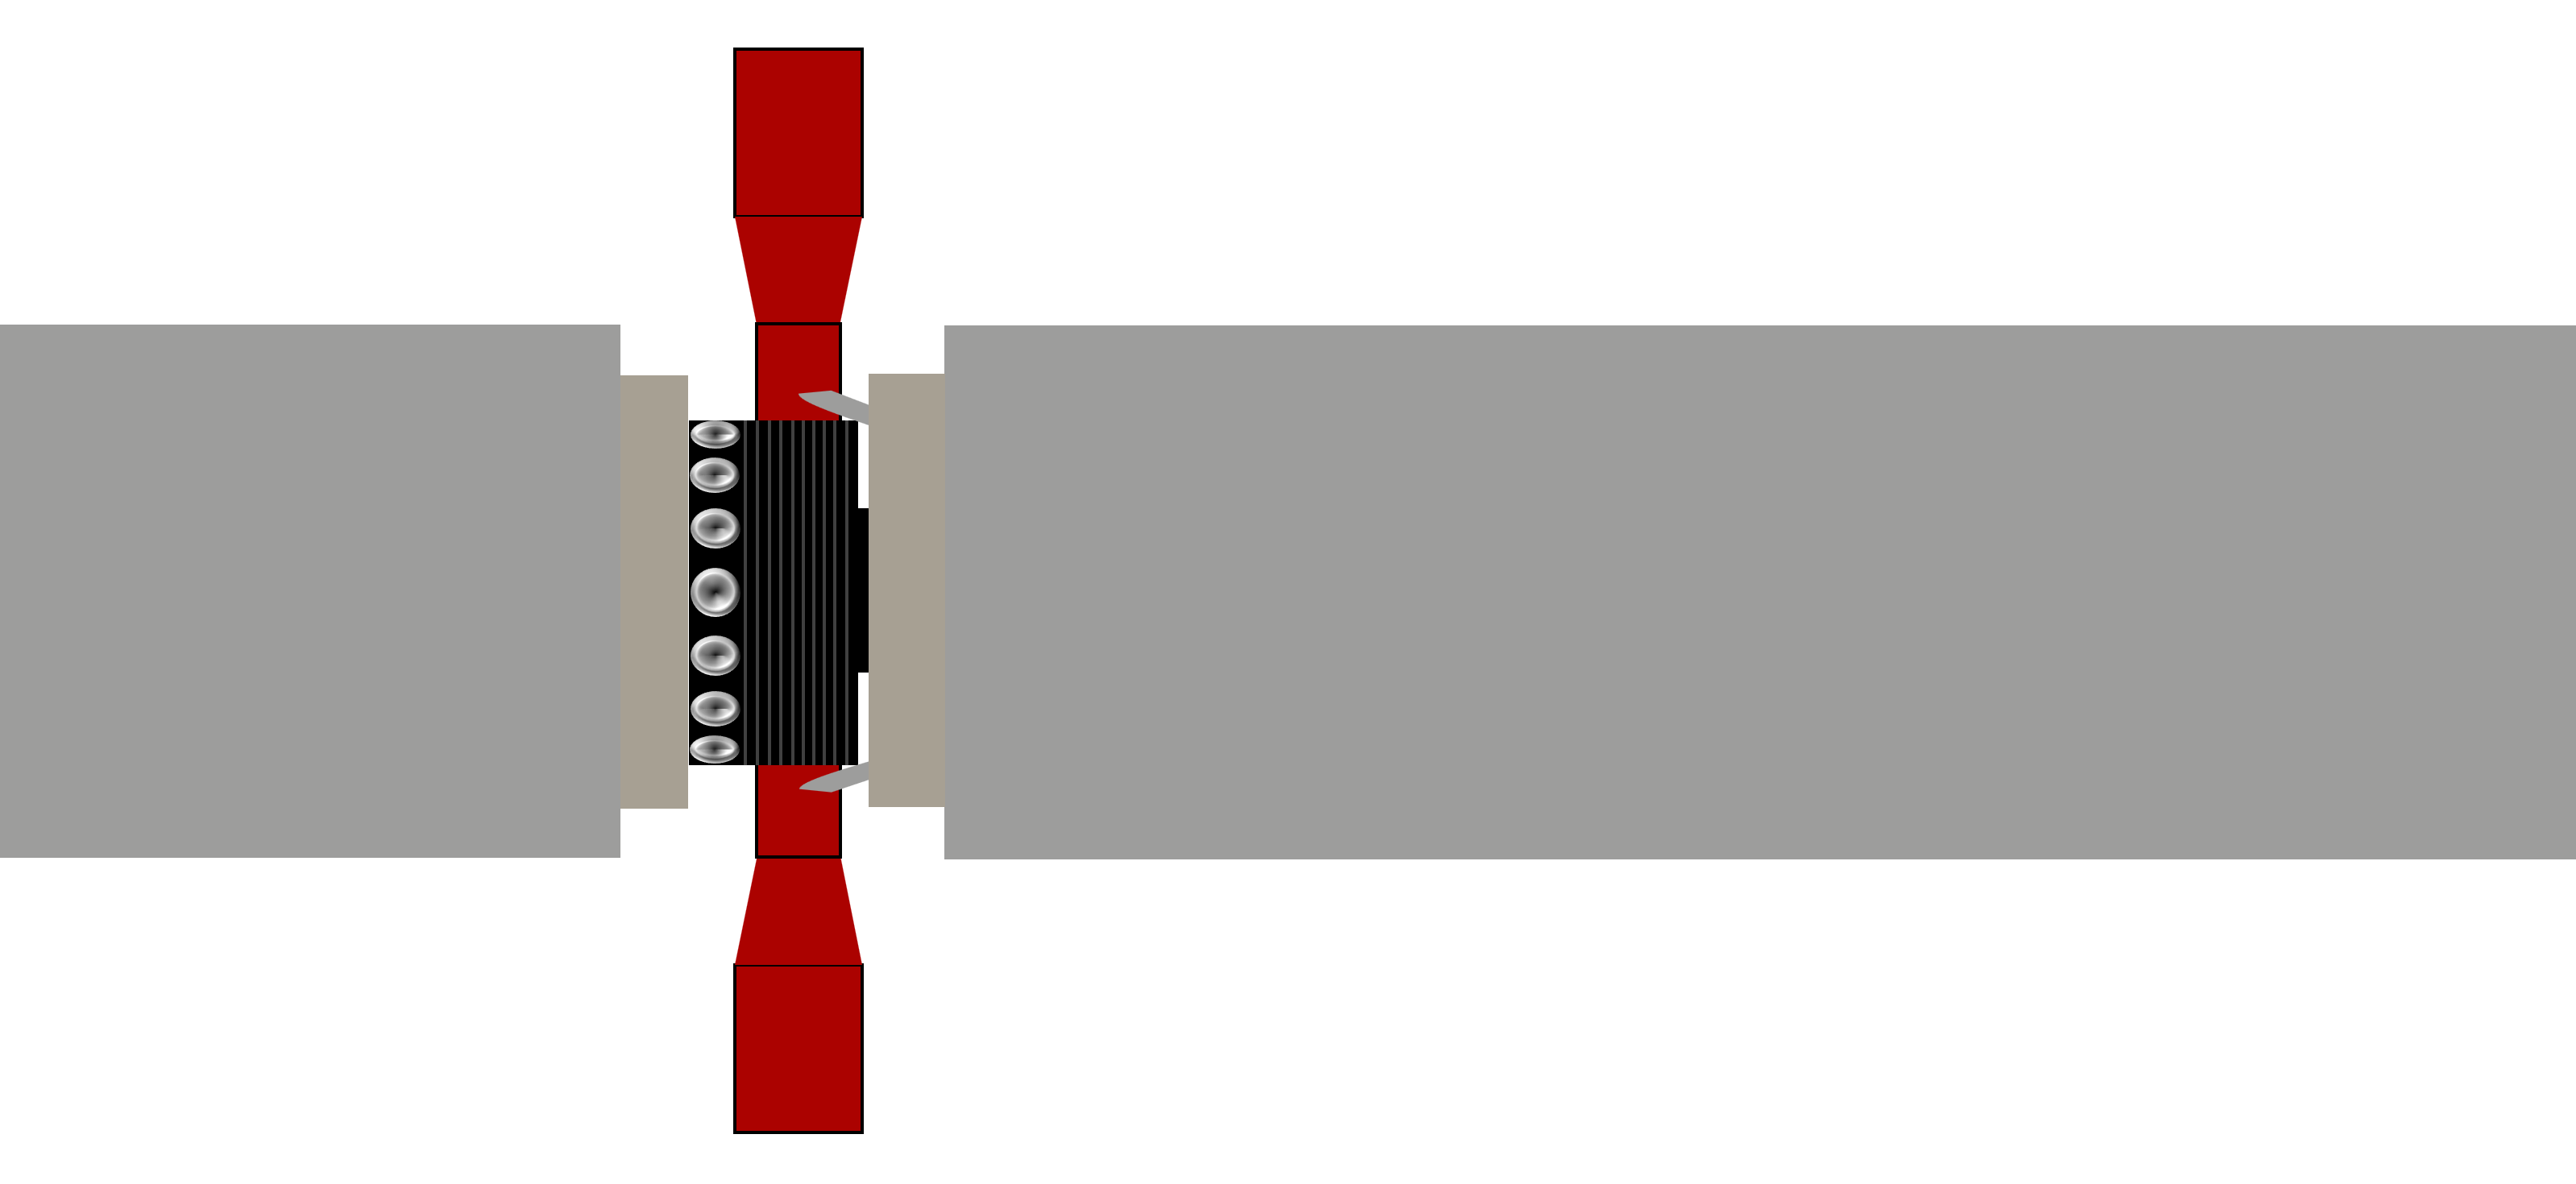
\includegraphics[width=\textwidth ]{images/lua_oop_ILUC_ribs.png}
        \caption{The laser line scanners detect the ILUC ribs. This can be used to further adjust the new joint's position,
            matching more closely the orientation of the main line.}
        \label{fig:oop_ILUC_ribs}
    \end{subfigure}
    \begin{subfigure}{0.7\textwidth}
        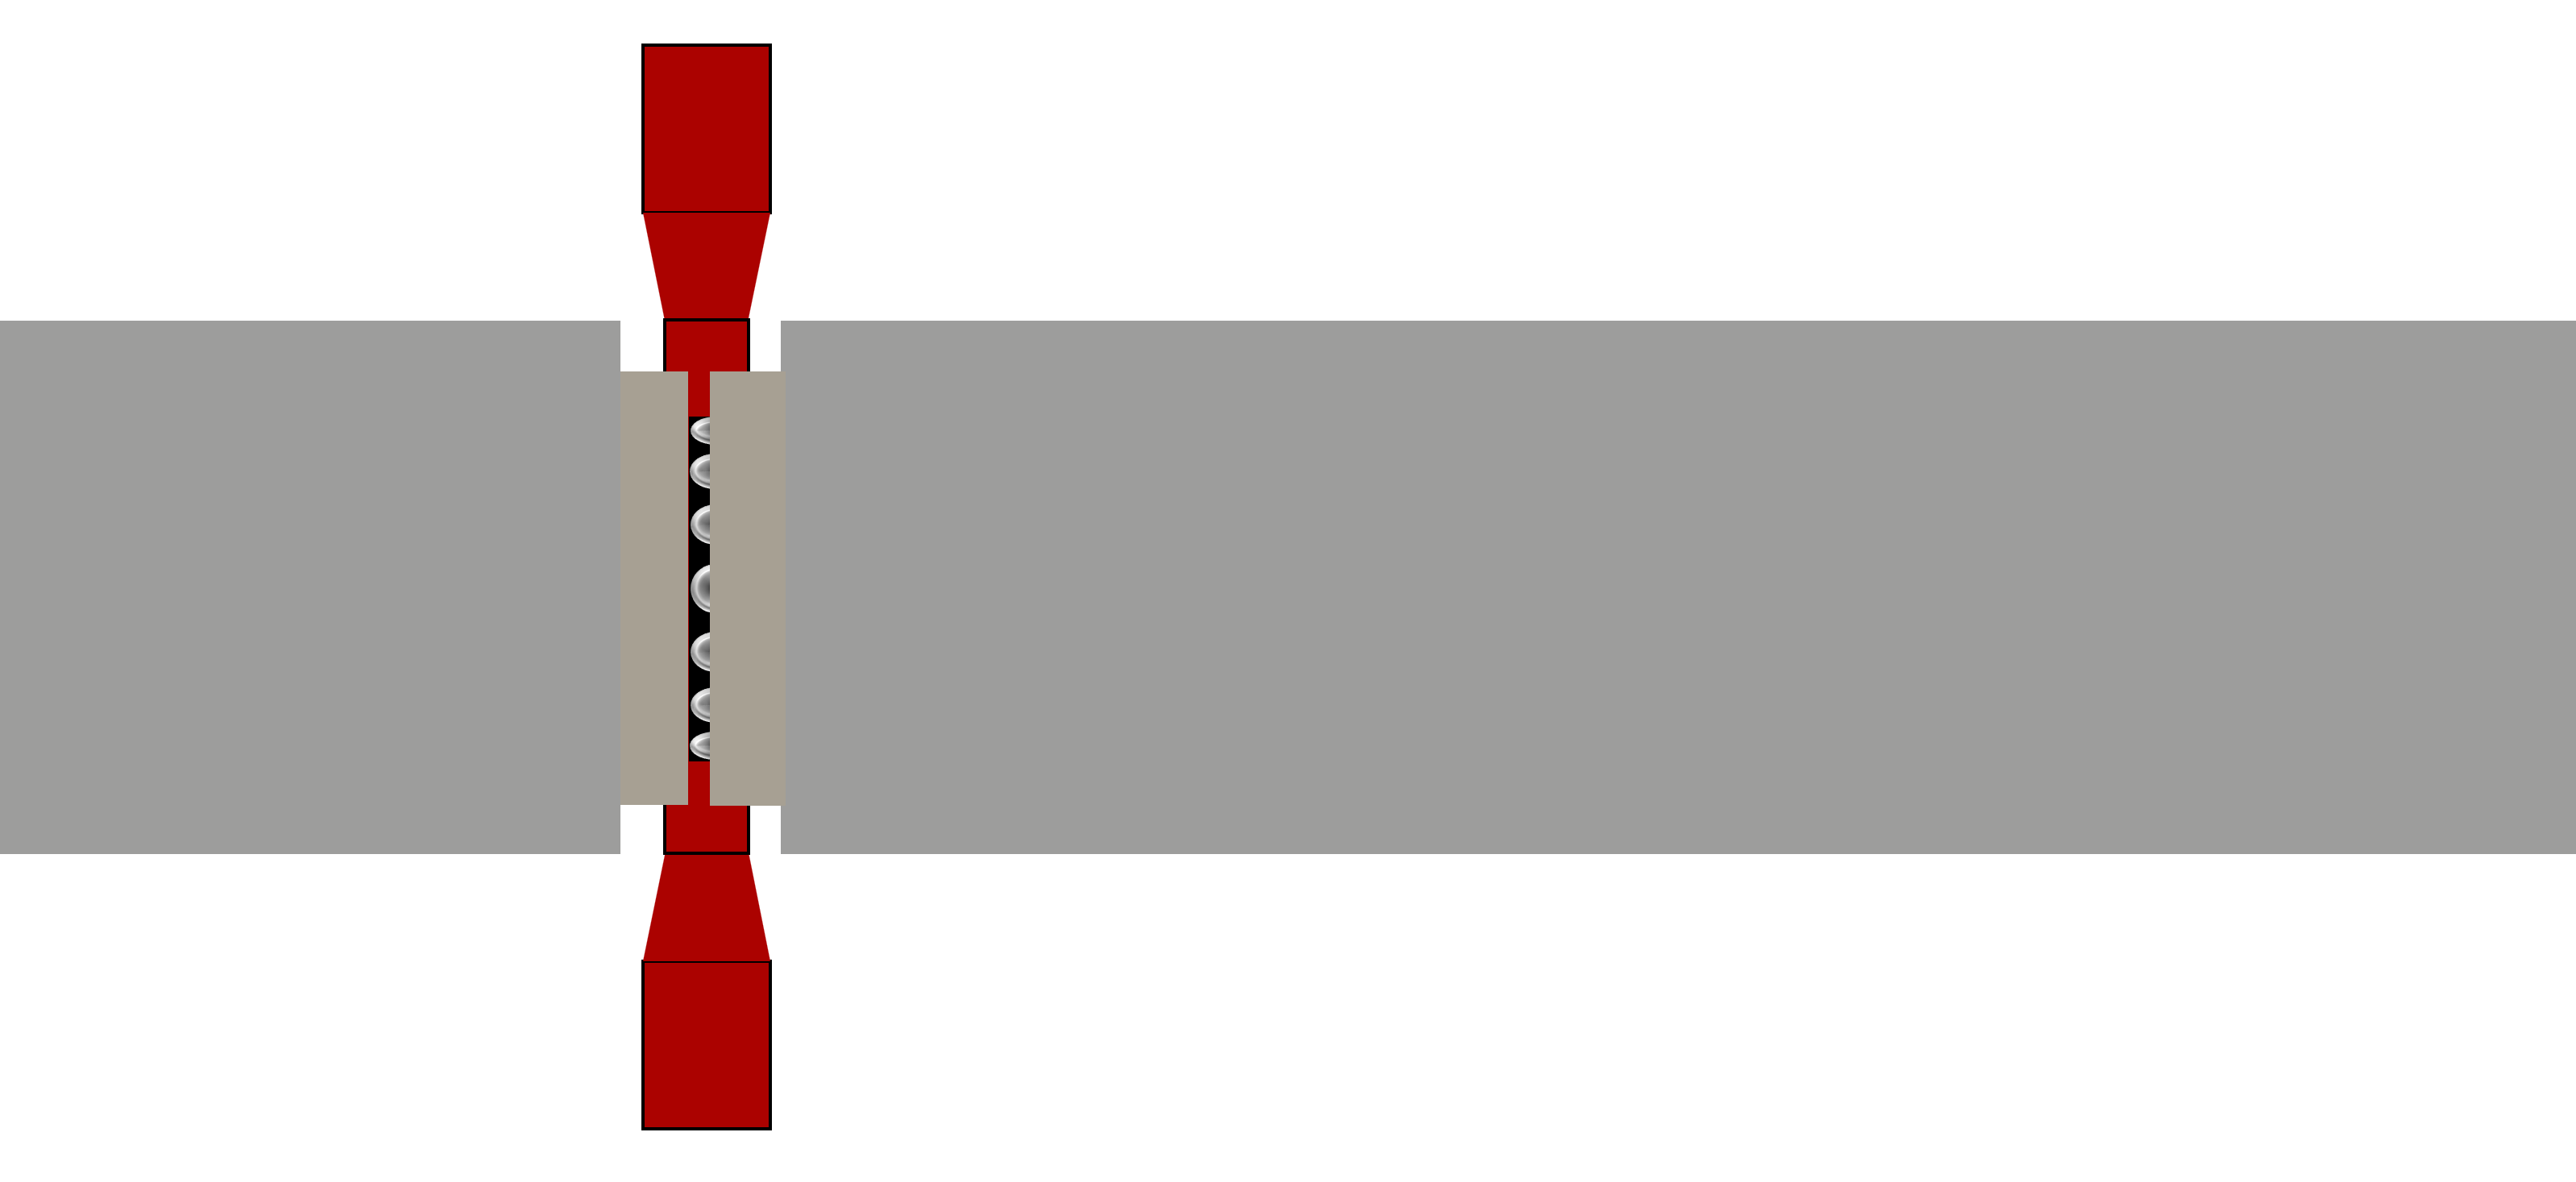
\includegraphics[width=\textwidth ]{images/lua_oop_final_line_up.png}
        \caption{Both pipe ends are fitted together during final line up. Adjustments are made to the new joint's position
            until a certain minimum gap tolerance is reached.}
        \label{fig:oop_final_line_up}
    \end{subfigure}
    \begin{subfigure}{0.7\textwidth}
        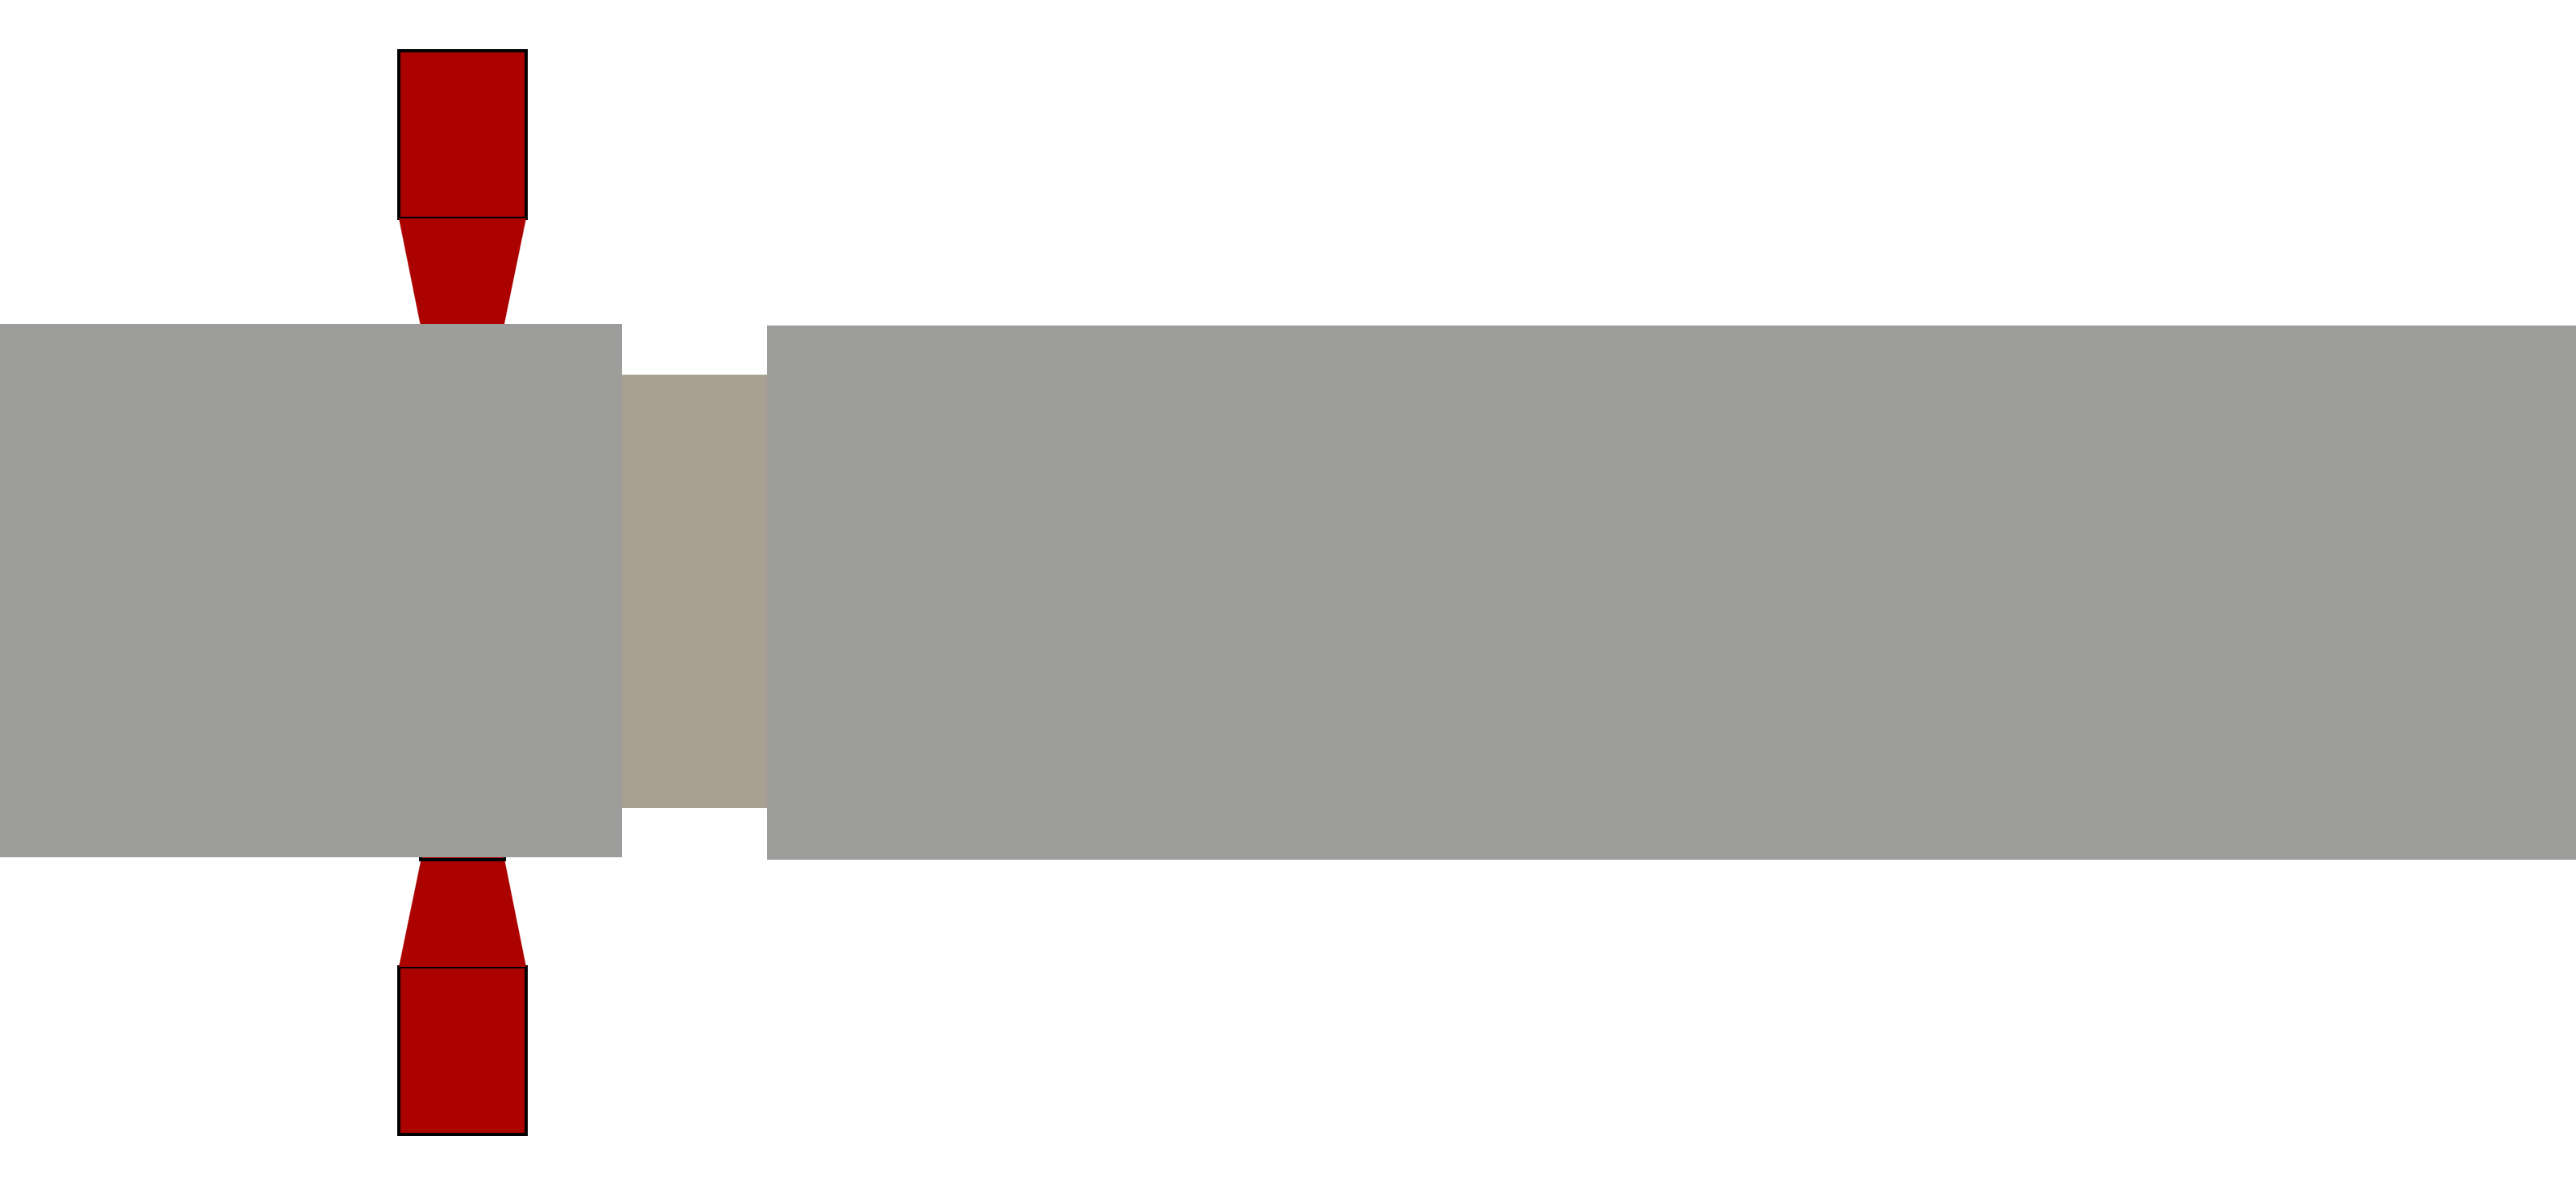
\includegraphics[width=\textwidth ]{images/lua_oop_end.png}
        \caption{U-Frame moves back to its starting position. The new joint is now fitted to the main line. The pipelines
            are now ready for welding.}
        \label{fig:oop_end}
    \end{subfigure}
    \caption{Simplified order of operations during automated line-up. This procedure is repeated for
        each new joint that is added to the main line. After final line up in \ref{fig:oop_final_line_up} is completed, the new joint
        is welded to the main line. Then, the whole pipeline is moved forward and the process is repeated for the next new joint.}
    \label{fig:oop_lua}
\end{figure}

Figure \ref{fig:oop_lua} offers only simplified overview of the automated line-up process.
Not shown in the figure are the;
\begin{enumerate}
    \item [-] \textbf{sub-frame}: system that controls the U-Frame's movements;
    \item [-] \textbf{laser line scanners}: sensors that detect the new joint's position;
    \item [-] \textbf{Line up Car Assemblies (LCAs)}: devices that precisely control the new joint's position and orientation;
\end{enumerate}

\newpage
\subsection{Flow of line up automation software} \label{ssec:code_flow}
The code flow of the laser line scanner software is shown in figure \ref{fig:code_flow}. This is an high-level
overview of the software's operation.
\begin{figure}[H]
    \centering
    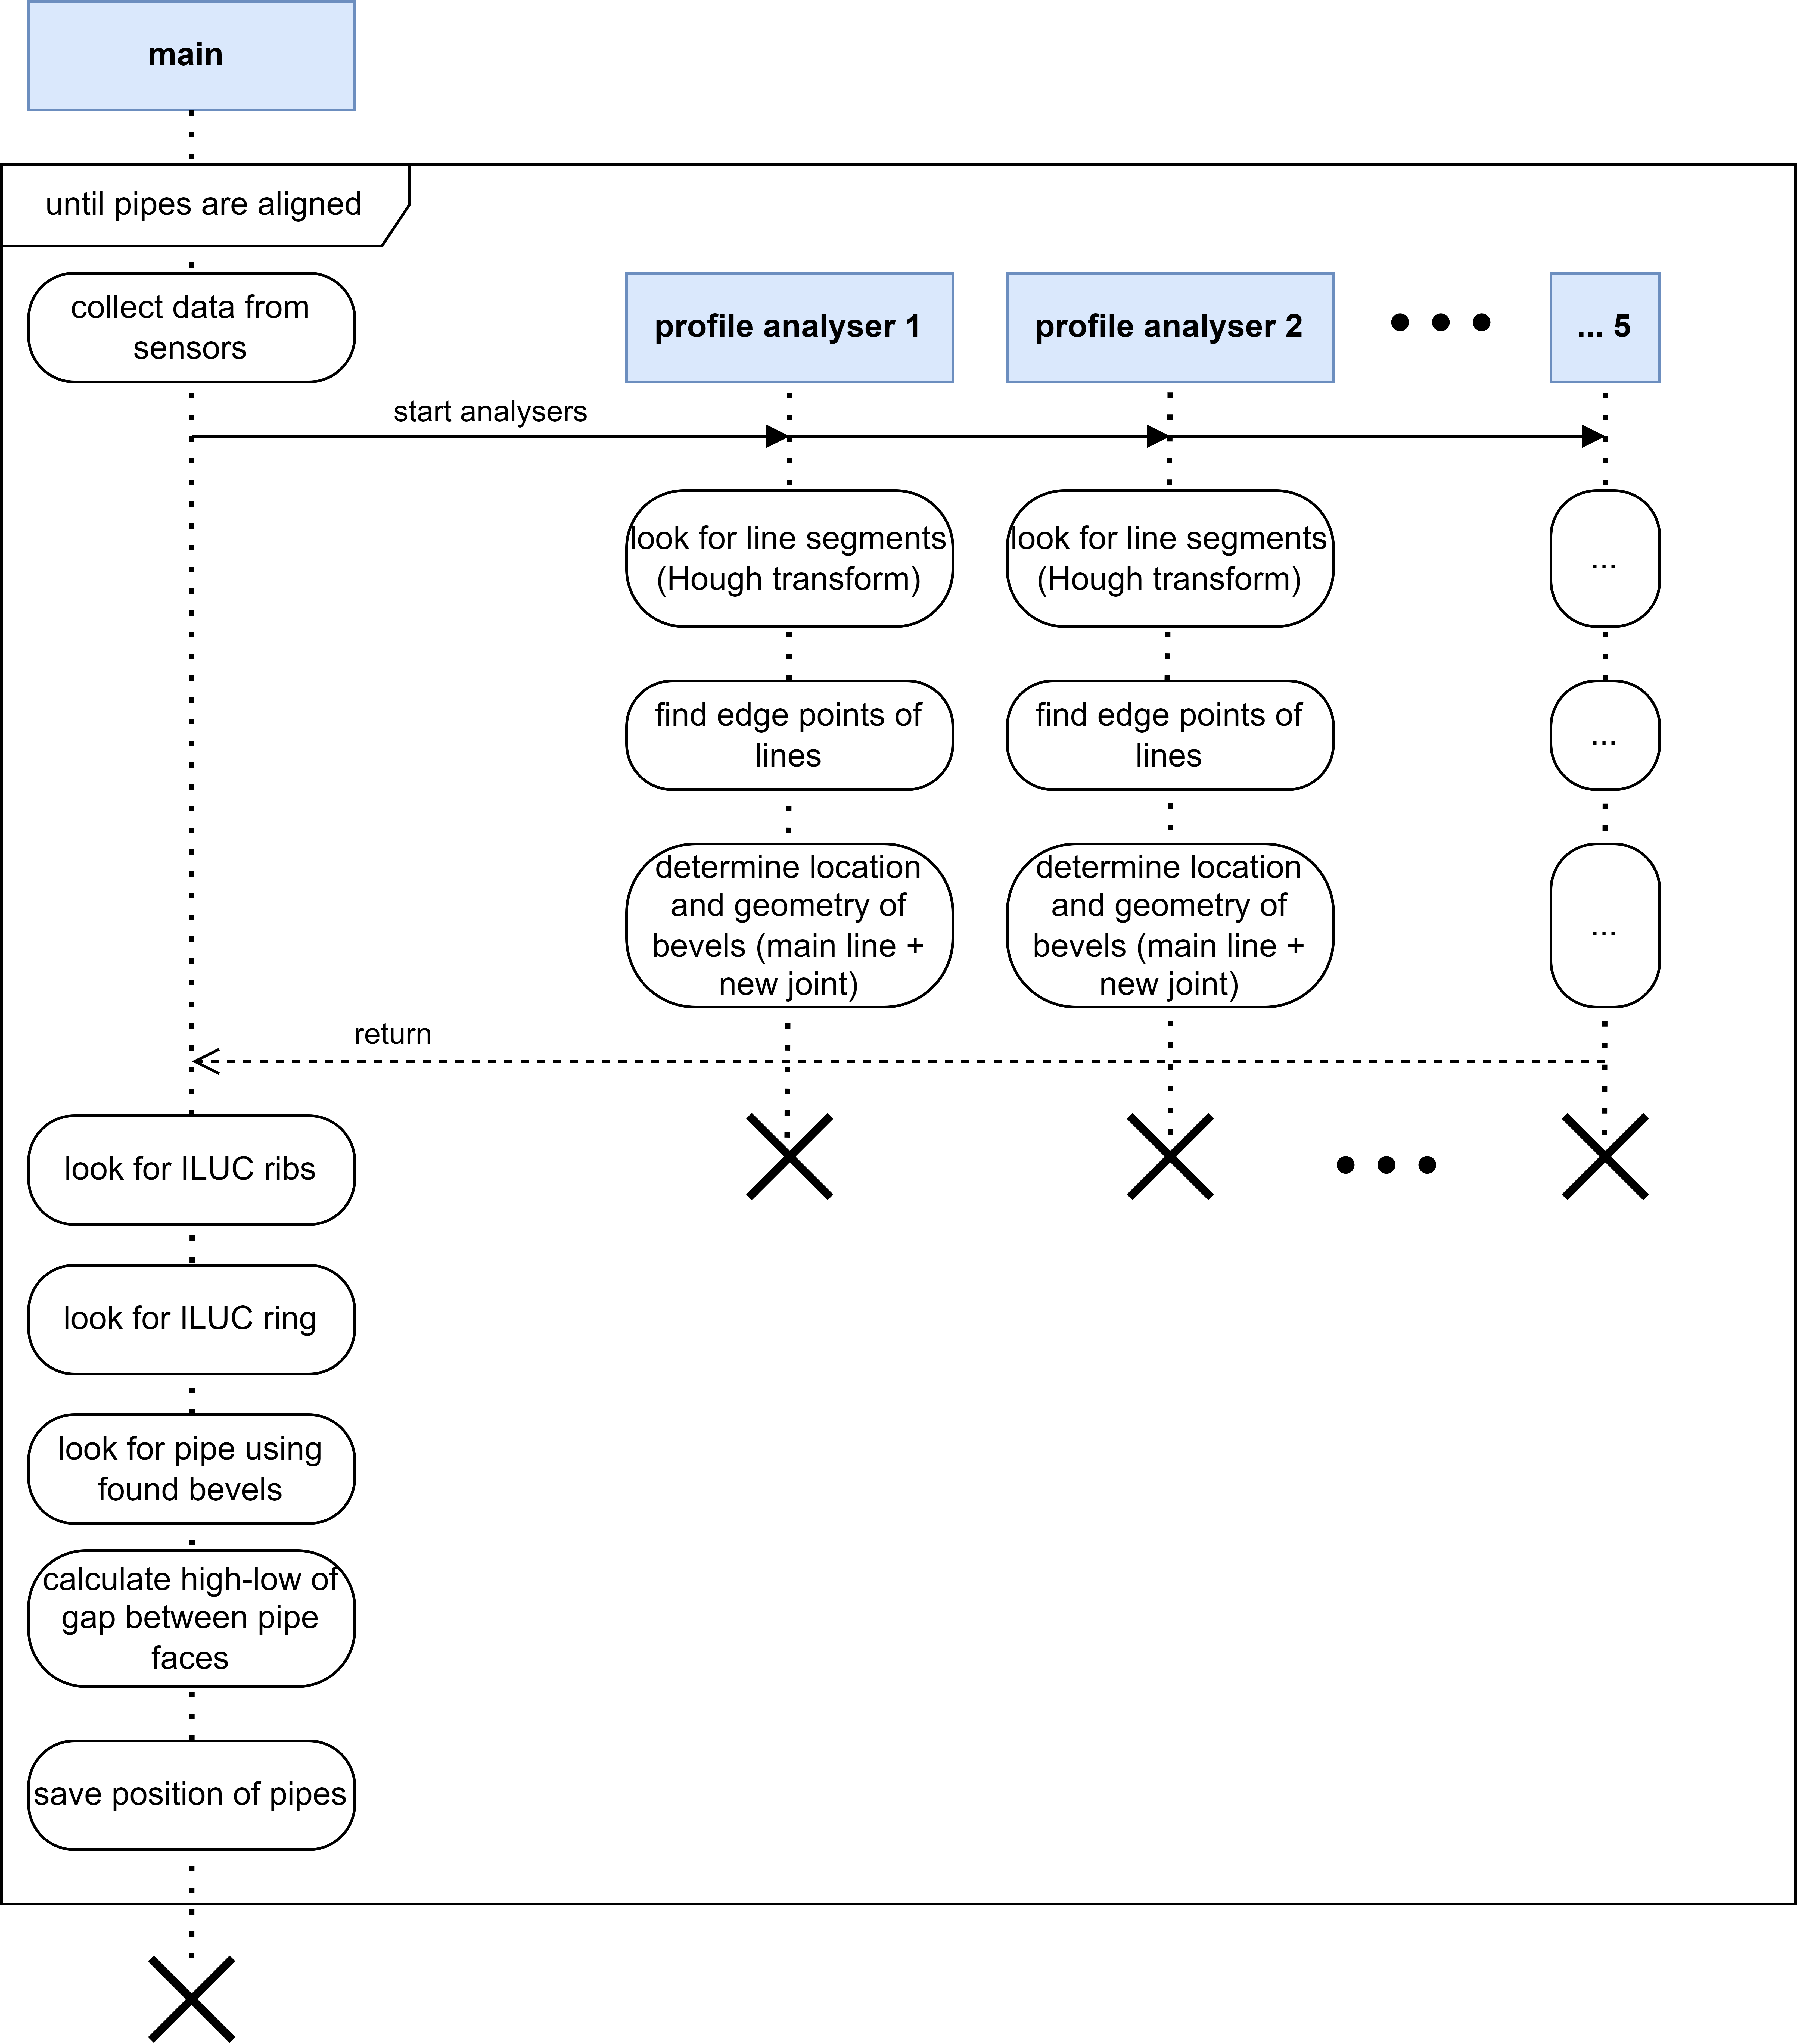
\includegraphics[width=\textwidth]{images/automated_lineup_flow.png}
    \caption{Flow of the laser line scanner software. The software is a multithreaded application. The blue boxes
        with bold text indicate the birth of these threads. The dotted lines are the `life-lines' of the threads, which always terminate in an
        `$\times$'. The frame symbolises the main loop of the software. The top-left compartment in the frame
        specifies the loop-condition; `until pipes are aligned'. The rounded boxes on the life-lines indicate functions that are called. Note that only
        the main thread can call functions. The main thread is responsible for the initialisation of the software and the creation of the other threads.}
    \label{fig:code_flow}
\end{figure}
As can be seen in figure \ref{fig:code_flow}, the laser line scanner software assigns a seperate thread for the analysis of the data coming from each of the five laser line scanners. These analyser threads are responsible for finding line-segments, edge points and pipe bevels in their respective 2-dimensional data sets. Once this preliminary, disjoint analysis is done, the main thread combines the processed data into a 3-dimensional model of the ILUC ribs, -ring and/or pipes. Specifically, the models for the pipes are used to calculate the high-low values of the gap between the new joint and the main line. The high-low values determine if the pipes are lined-up correctly. If the gap is within a certain tolerance, the software will signal that the pipes are aligned and it terminates the main loop.

Comparing Figures \ref{fig:oop_lua} and \ref{fig:code_flow}, it becomes clear that the relative activity of the various parts of the software change
depending on the stage of the automated line-up process. For example, determining the location and geometry of a pipe's bevel is only necessary as soon as
the new joint comes into Field of View (FOV) of the laser line scanners (step \ref{fig:oop_track}). Then, the activity roughly doubles as soon as the main line
comes into FOV of the laser line scanners during final line up (step \ref{fig:oop_final_line_up}). Furthermore, the finding of lines and their edges in each of the profile analyser threads becomes more computationally expensive for the ILUC ribs. This is further explored in section \ref{sec:profiler}.